% !TEX TS-program = pdflatex
% !TEX encoding = UTF-8 Unicode

% This is a simple template for a LaTeX document using the "article" class.
% See "book", "report", "letter" for other types of document.

\documentclass[11pt]{article} % use larger type; default would be 10pt

\usepackage[utf8]{inputenc} % set input encoding (not needed with XeLaTeX)

%%% Examples of Article customizations
% These packages are optional, depending whether you want the features they provide.
% See the LaTeX Companion or other references for full information.

%%% PAGE DIMENSIONS
\usepackage{geometry} % to change the page dimensions
\geometry{letterpaper} % or letterpaper (US) or a5paper or....
% \geometry{margins=2in} % for example, change the margins to 2 inches all round
% \geometry{landscape} % set up the page for landscape
%   read geometry.pdf for detailed page layout information

\usepackage{graphicx} % support the \includegraphics command and options

% \usepackage[parfill]{parskip} % Activate to begin paragraphs with an empty line rather than an indent

%%% PACKAGES
\usepackage{booktabs} % for much better looking tables
\usepackage{array} % for better arrays (eg matrices) in maths
\usepackage{paralist} % very flexible & customisable lists (eg. enumerate/itemize, etc.)
\usepackage{verbatim} % adds environment for commenting out blocks of text & for better verbatim
\usepackage{subfig} % make it possible to include more than one captioned figure/table in a single float
\usepackage{amsmath}
\usepackage{amssymb}
% These packages are all incorporated in the memoir class to one degree or another...

%%% HEADERS & FOOTERS
\usepackage{fancyhdr} % This should be set AFTER setting up the page geometry
\pagestyle{fancy} % options: empty , plain , fancy
\renewcommand{\headrulewidth}{0pt} % customise the layout...
\lhead{}\chead{}\rhead{}
\lfoot{}\cfoot{\thepage}\rfoot{}

%%% SECTION TITLE APPEARANCE
\usepackage{sectsty}
\allsectionsfont{\sffamily\mdseries\upshape} % (See the fntguide.pdf for font help)
% (This matches ConTeXt defaults)

%%% ToC (table of contents) APPEARANCE
\usepackage[nottoc,notlof,notlot]{tocbibind} % Put the bibliography in the ToC
\usepackage[titles,subfigure]{tocloft} % Alter the style of the Table of Contents
\renewcommand{\cftsecfont}{\rmfamily\mdseries\upshape}
\renewcommand{\cftsecpagefont}{\rmfamily\mdseries\upshape} % No bold!

%%% END Article customizations

%%% The "real" document content comes below...

\title{CS267 Assignment 2}
\author{Patrick Li, Simon Scott, Stephen Twigg}
%\date{} % Activate to display a given date or no date (if empty),
         % otherwise the current date is printed 

\begin{document}
\maketitle
\parskip 7.2pt

\section{Introduction}

The aim of this assignment was to develop parallel implementations of a particle simulator, using both shared memory and distributed memory systems. This was achieved by first developing serial implementations of the collision detection algorithm that ran in O(n) time. Two serial implementations were written: one using micro-blocks and one using a prune-and-sweep algorithm. These serial implementations were then parallelized using the MPI, OpenMP, Pthreads and CUDA frameworks.

Each of these serial and parallel algorithms are described in Section \ref{algorithm-section}, and their performance is analyzed in Section \ref{results-section}. Finally, Section \ref{conclusion-section} draws conclusions from these results.


%%%%%%%%%%%%%%%%%%%%%%%%%%%%%%%%%%%%%%%%%%%%%%%%%%
%%%% ALGORITHMS SECTION                       %%%%
%%%%%%%%%%%%%%%%%%%%%%%%%%%%%%%%%%%%%%%%%%%%%%%%%%


\section{Description of Algorithms}
\label{algorithm-section}

The micro-blocks and prune-and-sweep algorithms for collision detection are described below. This is then followed by a discussion of how these algorithms were extended to parallel implementations.

\subsection{Serial Micro-blocks}

The microblocking algorithm divides the simulation space into square blocks with side-lengths proportional to {\em cutoff}. After particle creation, each particle is assigned to a corresponding microblock. For each particle, we find its colliding neighbours by checking against all other particles in its own and neighbouring microblocks. Since the forces are repulsive and the particle density is $\sim$1/2 particles per $\text{\em cutoff}^\text{~2}$, there are on average a small number of particles within each microblock. We explored a variety of microblock sizes and found that microblocks with side-lengths of $2\times\text{\em cutoff}$ to be optimal, corresponding to roughly 2 to 3 particles per block. Thus, during collision detection, each particle must check against roughly 21 other particles. A full collision detection sweep is done in $O(n)$ time. Calculating the force on each particle, updating its position, and assigning it to its new microblock is done independently for each particle, and thus takes $O(n)$ time.

Small optimizations were used to speed up this microblocks implementation. Rather than actually store the particle data in the microblocks, the particle list simply contains addresses to particles in a global particle array. This allows microblock assignment to be done by simply moving single pointers around instead of moving an entire particle data structure. The microblock particle list is modeled after STL vectors and thus insertions and deletions take O(1) time. Similar to STL vector, the particle list is capable of expanding to greater sizes as needed; however, for the particle counts we simulated, a microblock rarely contained more than 4 particles. New microblock assignments are calculated by dividing its position by the microblock sizes in order to handle the case where particles jump across entire microblocks within a single time step,

\subsection{Serial Sweep and Prune}

Particle simulations with only near-field effects have two major characteristics
that can be exploited when optimizing for performance:
\begin{enumerate}
\item Spatial Locality: A particle only interacts with its nearby neighbours.
\item Temporal Locality: If two particles are nearby in the current timestep,
they are likely to be nearby in the next timestep.
\end{enumerate}
Sweep and Prune is a collision detection algorithm that exploits temporal
locality. The algorithm internally maintains two sorted lists, one
list containing the particles sorted by their x coordinates, and another
list containing the same particles but sorted by their y coordinates.
Particles that are distant with regards to their list position are
unlikely to be colliding. Furthermore, if particles have not moved
too great a distance since the last timestep then the lists will remain
\emph{nearly} sorted. A sort routine with complexity proportional
to the orderedness of the list, such as insertion sort, is then used
to keep the lists sorted efficiently. 

\subsubsection{Algorithm Initialization}

Here, the simple case of collision detection in 1D is used to explain
the basic algorithm. Generalizing the algorithm to $N$ dimensions
is straightforward and discussed later. The algorithm initially starts
with an initially empty list, $L$. For each object $o_{i}$, we add
two tokens, $\text{MIN}_{i}$ and $\text{MAX}_{i}$, to the end of
$L$, where $\text{MIN}_{i}$ is the tuple $(\text{MIN},i,x_{\text{i},\text{min}})$
and $\text{MAX}_{i}$ is the tuple $(\text{MAX},i,x_{\text{i},\text{max}})$.
$\text{MIN}$ and $\text{MAX}$ are labels that indicate the type
of the token. $i\in\{1,\ldots,N\}$ is the index of the object. $x_{\text{i},\text{min}},x_{\text{i},\text{max}}\in\mathbb{R}$,
are the x coordinates of the left-hand and right-hand boundaries of
the object respectively. A mapping $M$
from unordered pairs of indices to booleans, $M:(i,j)\in\{1,\ldots,N\}^{2}\rightarrow\text{bool}$, is maintained to indicate whether object $i$ and $j$ are intersecting. $M$
is initially false for every pair $i$ and $j$.

\subsubsection{Update Step}

To detect collisions, we use an insertion sort to sort L according
to the x coordinates of the tokens. 

\[
\begin{aligned} & \text{for }k\text{ in }0\ldots2N\text{ do : }\\
 & \quad m\text{ := }k\\
 & \quad\text{while }m>1:\\
 & \quad\quad\text{if }L_{m-1}.x<L_{m}.x:\\
 & \quad\quad\quad\text{swap}(m,m-1)\\
 & \quad\quad\quad m=m-1\\
 & \quad\quad\text{else :}\\
 & \quad\quad\quad\text{break}
\end{aligned}
\]
where the function \emph{swap} interchanges the positions of token
$m$ and token $m-1$, and updates the mapping $M$. If the $\text{MAX}$
token of object $i$ is swapped to the right of the $\text{MIN}$
token of object $j$ then we set $M(i,j)$ to $\text{true}$, to indicate
that object $i$ is now intersecting with object $j$. If the $\text{MIN}$
token of object $i$ is swapped to the right of the $\text{MAX}$
token of object $j$ then we set $M(i,j)$ to $\text{false}$ to indicate
that object $i$ is no longer intersecting with object $j$. 

\[
\begin{aligned} & \text{define swap }(i,j):\\
 & \quad\text{if }L_{i}\text{.type}=\text{MIN and }L_{j}\text{.type}=\text{MAX}:\\
 & \quad\quad M(i,j)=\text{true}\\
 & \quad\text{else if }L_{i}\text{.type}=\text{MAX and }L_{j}\text{.type}=\text{MIN}:\\
 & \quad\quad M(i,j)=\text{false}\\
 & \quad\text{interchange }L_{i}\text{ with }L_{j}
\end{aligned}
\]
At the end of the sort stage, and $L$ is properly sorted, $M(i,j)$
will indicate whether the bounding boxes of object $i$ intersects
with object $j$. The very first timestep will take $O(N^{2})$ time
because there is no guarantee on the initial ordering of $L$. But
for all subsequent timesteps, if the timestep is small and particles
do not move excessively, the sort can be completed in close to $O(N)$
computations. As a further possible optimization, a quick $O(n\cdot\text{log }n)$
sort can be used to obtain the initial ordering for $L$. We do not include the list construction and initial sort in our timings.

\subsubsection{Generalization to N-D}

To generalize the single dimensional sweep and prune algorithm to
$N$ dimensions, we now maintain $N$ sorted lists. We note that the
bounding boxes of objects $i$ and $j$ are overlapping if and only
if they are overlapping in all $N$ dimensions. Thus at each timestep
we perform $N$ sorts, and check that $M(i,j)=\text{true}$ for each
dimension. 

\subsection{MPI using Micro-blocks}

To parallelize the microblocks algorithm, we first coursely subdivide the simulation space into regions, and assign each region to a separate processor. Analogously to microblocks, regions send particles near the border to neighbouring regions as ghosts, and a region checks for collisions between all owned particles and ghost particles. Particles are migrated across region boundaries as needed. Within a single region, we use the serial microblocks implementation.

To determine which particles need to be sent as ghosts to neighbouring regions, we scan through the microblocks near the border of the regions. Since we must iterate through all particles in a microblock anyway to determine which particles to migrate, we can, at this time, also check whether they need to be sent as ghosts to neighbouring regions. To prevent unnecessary copying of data we store only pointers to particles in the microblocks, and to prevent recomputing its neighbours on each frame each microblock also stores pointers to neighbouring microblocks.

\subsection{MPI using Sweep and Prune}

The physical particle space is divided into a 2D grid, with each block in the grid assigned to a different processor. Initially, processor 0 broadcasts all the particles to all other processors. Each processor then selects the particles that fall within its ``physical'' boundaries, and adds these particles to a local, sorted, particle list.

After the initialization stage, the main loop performs the following operations, in order. Note that each processor has a list of its own particles, as well as the ghost particles that lie in the regions immediately surrounding the processor.
\begin{itemize}
\item Calculate the forces on local particles, due to other local particles, as well as ghost particles.
\item Move the local particles, using the sweep and prune algorithm to determine collisions between the local and ghost particles.
\item Determine which local particles have moved outside the boundaries of this processor. Use MPI to send these emigrant particles to the relevant neighboring processor. Similarly, immigrant particles, which have now moved into this processor's space, are received from neighbors and added to the local sorted list.
\item Determine which local particles lie near the (inside) boundary of this processor. These are the ghost particles, and are sent to neighboring processors in MPI messages.
\item Receive ghost particles from neighboring processors, and sort them into the local particle list.
\end{itemize}

Emigrant particles are sent to all eight neighboring processors using an asynchronous MPI send, and then removed from the local list of particles. The processor then does a blocking read from each of its eight neighbors, in turn. When the list of immigrant particles is received from each neighbor, these particles are sorted into the local list of particles. This sorting process may be costly if there are lots of immigrants. The blocking reads are essentially the synchronization step in this algorithm. However, to ensure that all processors do in fact stay in synchronization, an MPI {\em Waitall} command is also used.

Besides determining the emigrant particles that must leave the processor, each processor also determines which local particles lie near the boundary of, but still within, the processor's space. The particles that lie within this ghost region are added to one of three lists: new ghost list (if they were not within the ghost region last cycle), moved ghost list (if they were within the ghost region last cycle) or the deleted ghost list (if a particle is no longer a ghost). These three lists are then sent to the appropriate neighbors, with an asynchronous MPI send.

Each processor then performs three blocking reads from each of its neighbors, to receive the three ghost lists. Each ghost particle is either added, removed or moved around in the local particle list. The advantage of having three lists is that particles tend to remain in the ghost region for a number of consecutive cycles, and simply updating the position of the ghost particles is much faster O(1) than removing and then adding the ghost particles back O(n).

If the results must be saved, an MPI Gather operation is used to send all the particles to processor 0, who writes them to file.

\subsection{Pthreads using Sweep and Prune}
The Sweep and Prune algorithm maps well onto sequential hardware but
parallelization across multiple processors is difficult. We opted to
parallelize sweep and prune by partitioning the simulation space into
separate regions and assigning each region to a separate processor.
Within a single processor we use the sequential sweep and prune algorithm. 


\subsubsection{Regions}

A region structure contains fields that indicate the extents of its
boundaries, $\text{min}_{x},\text{max}_{x},\text{min}_{y},\text{max}_{y}$,
pointers to its neighbouring regions, and a local sweep and prune
structure for managing the particles local to the region. Particles
may only be added or removed from a region using the \emph{add\_region\_particle
}and \emph{remove\_region\_particle} functions.


\subsubsection{Region Bounds}

Regions have several bounds for the purposes of partitioning the workload
amongst processors. $\text{min}_{x},\text{max}_{x},\text{min}_{y},\text{max}_{y}$
define the \emph{responsibility bounds}. A region is responsible for
correctly computing the forces and updating the positions of all particles
within its \emph{responsibility bounds.} The \emph{send bounds }of
a region starts at a distance of \emph{cutoff }interior from the border
and continues to the border. Any particles within the \emph{send bounds
}need to have its position sent to the neighbouring regions in order
for the regions to accurately compute collisions along boundaries.
The \emph{ghost bounds }of a region starts at the border and continues
to a distance of \emph{cutoff }exterior to the border. The region
will receive the positions of particles within the \emph{ghost bounds}
from neighbouring regions to use for handling collisions along the
boundaries.


\subsubsection{Algorithm}

Every region is run in its own thread of execution, and at every time
step :
\begin{enumerate}
\item Determines which particles are in the \emph{send bounds} and need
to be sent to their neighbours.
\item Sends the particles to its neighbours. Particles are sent to each
neighbour (N, NE, E, SE, S, SW, W, NW) in turn, with a synchronizing
barrier after each. This barrier ensures that a region is receiving particles
from only one thread at a time.
\item Removes any particles that are outside its \emph{responsibility bounds.}
\item Computes forces and updates the positions of all particles within
its \emph{responsibility bounds.}
\end{enumerate}
The algorithm is summarized as :

\[
\begin{aligned} & \text{for timestep in }1\ldots\text{NSTEPS do :}\\
 & \quad\text{send\_particles := in\_sending\_bounds(all particles)}\\
 & \quad\text{barrier}\\
 & \quad\text{for neighbour in [N, NE, E, SE, S, SW, W, NW] do :}\\
 & \quad\quad\text{send\_to\_neighbour(neighbour, send\_particles)}\\
 & \quad\quad\text{barrier}\\
 & \quad\text{remove\_particles\_out\_of\_responsible\_bounds}\\
 & \quad\text{barrier}
\end{aligned}
\]

\subsection{OpenMP using Microblocks}

The OpenMP implementation uses the microblocks algorithm as it was found to be extremely easy to develop. In fact, the serial microblocks algorithm was chosen intentionally to serve as this a precursor to OpenMP. Only two major adjustments were required from the serial base. OpenMP pragmas were added to farm out particle collision detection/force calculation, particle movements, and particle migrations, all by microblock. Also, in the particle migration code, locks were added to the microblock particle lists to prevent possible race conditions when multiple threads add or remove particles from the same microblock simultaneously. Implicit barriers sit between the force calculation, movement, and migration stages due to features of the OpenMP for pragma feature.

\subsection{CUDA using Microblocks}

\subsubsection{The General Algorithm}

The sweep and prune algorithm would have required extensive modifications to port to a GPU architecture due to its inherently serial nature. For this reason, the GPU implementation uses the microblocks algorithm. Similarly to the OpenMP implementation, synchronization was needed to ensure proper behavior when multiple threads add/remove particles to the same microblock. Implicit barriers between the force calculation, particle movement, and migration stages were handled by the CUDA stream implementation.

\subsubsection{GPU Synchronization Techniques}
After we update the positions of each particle, we need to check whether
their new positions are still within the bounds of their microblocks.
If not, then they need to be removed from the current microblock and
added to another. Because each particle is assigned its own thread,
a single microblock may have many threads attempting to add and remove
particles from it simultaneously. To coordinate these additions and
removals we use an atomic compare and swap operation with a valid
array.

Every microblock allocates an $M$ element slots array, $s$, that
can store up to $M$ particles, and internally maintains an $M$ element
valid array, $v$, that indicates the status of slot. Each element
in $v$ may hold one of the following settings:
\begin{itemize}
\item EMPTY: This indicates that there is currently no particle stored in
that slot.
\item ADDING: This indicates that we are currently in the process of adding
a particle to that slot.
\item FULL: This indicates that there is a particle stored in the slot.
\end{itemize}
Adding a particle consists of scanning through and looking for an
EMPTY slot. If found, then we set it's status to ADDING, and proceed
to store the particle into the slot. After the particle is stored,
we set the status of the slot to FULL. Adding a particle, $p$, is
illustrated by the following pseudocode.

\[
\begin{aligned} & \text{for }i\text{ in }1\ldots M\text{ do :}\\
 & \quad\text{v0}:=\text{cas}(v[i],\text{EMPTY},\text{ADDING})\\
 & \quad\text{if v0 }=\text{EMPTY :}\\
 & \quad\quad s[i]=p\\
 & \quad\quad v[i]=\text{FULL}\\
 & \quad\quad\text{break}
\end{aligned}
\]


Removing a particle does not require any synchronization, and only
requires that we set the appropriate element in the valid array, $v$,
to EMPTY.

The GPU simulation loops through three kernels, compute\_forces, move\_particles, and migrate\_particles, that each require the previous stage to finish before starting. Since CUDA 2.0, within a single stream, kernel calls implicitly block when they encounter a different kernel, thus we are guaranteed that the three stages start and finish in sequence. 

\subsubsection{GPU-Specific Optimizations}
\label{gpu-optimization-section}

The following GPU-specific optimizations were attempted:

\begin{itemize}
\item {\em Particle migration: } In the initial algorithm, each micro-block thread scanned the global particle list every cycle, checking the location of each particle, and adding the appropriate particles to the micro-block's particle list. This meant that the particle lists were rebuilt from scratch every cycle. Once we figured out how to use atomic operations, each microblock instead migrated emigrant particles to their new micro-block when they moved. Since only a small fraction of the particles move across micro-block boundaries each cycle, this meant that the particle lists did not have to be rebuilt every cycle.

\item {\em Single kernel: } Currently, three separate kernels are used to compute forces, move particles, and migrate particles. An attempt was made to combine these three kernels into a single macro-kernel, with {\em \_\_sync\_threads()} operations between the compute, move and migrate stages of computation.

\item {\em Vector datatypes and local particle copy: } The particle position, velocity and acceleration values are stored using {\em double2} vector datatypes, to coalesce memory accesses. Also, if a kernel performs multiple operations on a particle, it copies the particle from global memory into its registers or local memory, modifies the particle, and then copies it back to global memory at the end.

\item {\em Per-particle threads for calculating forces: } Initially, when computing forces, a separate thread was launched for each micro-block. This thread computed the forces between all the particles in the micro-block, and the neighboring microblocks. The disadvantage of this is that the threads that are launched for empty microblocks are wasted computation. Therefore, a thread is instead launched for every particle in the system. This thread determines its micro-block, and computes the forces between itself and all other particles in its (and neighboring) microblock.

\item {\em Future work: shared memory: } A future optimization to the force calculation would be to arrange the thread launches so that all particles in a ``macro-block'' of micro-blocks run in the same thread block (or physical streaming multiprocessor). Each thread would then load its particle data from global memory into the shared memory. Since all the particles on the streaming multiprocessor are located near each other, they can read the position of all surrounding particles directly from shared memory. This would speed up memory accesses many-fold, and potentially speed up computation 2X-4X.
\end{itemize}



%%%%%%%%%%%%%%%%%%%%%%%%%%%%%%%%%%%%%%%%%%%%%%%%%%
%%%% RESULTS SECTION                          %%%%
%%%%%%%%%%%%%%%%%%%%%%%%%%%%%%%%%%%%%%%%%%%%%%%%%%


\section{Results}
\label{results-section}

The performance of the algorithms described in the previous section is reported here. The scaling of execution time with number of particles and number of processors is given, as well as how this execution time is allocated to the different parts of each algorithm.

\subsection{Serial Micro-blocks}

Figure~\ref{serial_mb_n} verifies the serial microblocks implementation is of O(n). The drop in performance for very high particle counts is most likely due to memory cache issues rather than algorithmic failure. Figure~\ref{serial_mb_flops} provides evidence to this theory as the floating point utilization (measured using CrayPAT) drops considerably as n increases. Even so, the latter figure demonstrates this problem is largely memory bound instead of compute bound, with most time spent setting up collision detection and comparing particle rather than actually calculating forces.

\begin{figure}[!h]
\centering
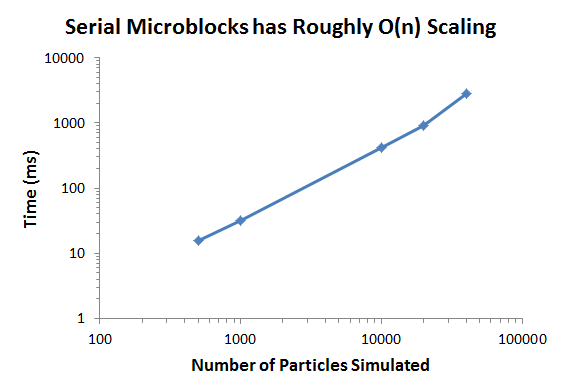
\includegraphics[width=0.65\textwidth]{figures/serial_mb_n.png}
\caption{}
\label{serial_mb_n}
\end{figure}

\begin{figure}[!h]
\centering
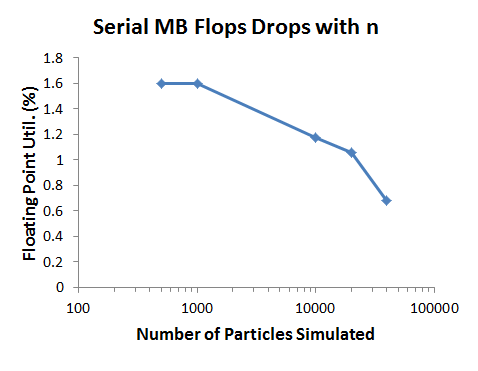
\includegraphics[width=0.65\textwidth]{figures/serial_mb_flops.png}
\caption{}
\label{serial_mb_flops}
\end{figure}

\subsection{Serial Sweep and Prune}

Figure \ref{plot:serial_t_v_n} shows how the execution time scales
with the number of particles for the serial prune and sweep algorithm.
Time is measured for $n=500,1000,10000,20000,\text{ and }40000$ particles
and plotted on a log-log pot. Fitting a trendline through the points
results in a line with slope \textasciitilde{}1.4. Although the total
computation time is an order of magnitude lower than the naive $O(n^{2})$
algorithm, the algorithm does not scale linearly with the number of
particles. The Sweep and Prune algorithm scales with the orderedness
of the x and y lists between frames and we see that as the number
of particles increase, the lists are less likely to remain sorted. 

\begin{figure}
\begin{centering}
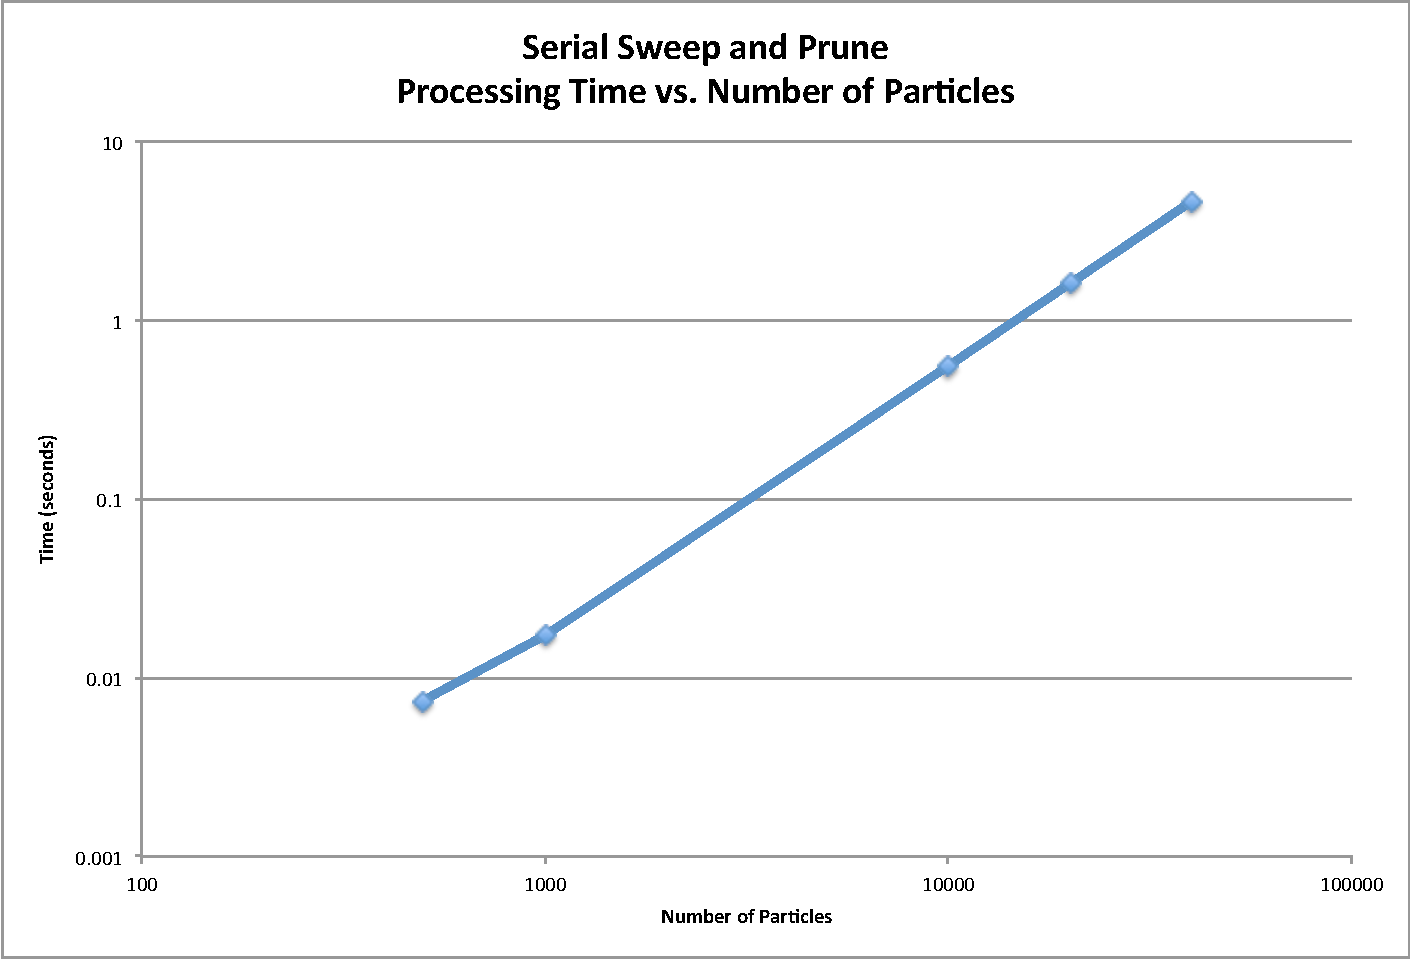
\includegraphics[width=0.5\paperwidth]{figures/serial_t_v_n}
\par\end{centering}

\caption{Serial Sweep and Prune. Time versus Number of Particles.}
\label{plot:serial_t_v_n}

\end{figure}


Figure \ref{plot:serial_flops_v_n} shows how the number of floating
point operations scale with the number of particles, $n=500,1000,10000,20000,\text{ and }40000$.
We see that as the number of particles increase the number of floating
point operations decrease drastically. This is to be expected as the
orderedness of the lists decrease with the increase in number of particles.
Thus the execution time is increasingly dominated by the sort required
by sweep and prune than by the force and position updates.

\begin{figure}
\begin{centering}
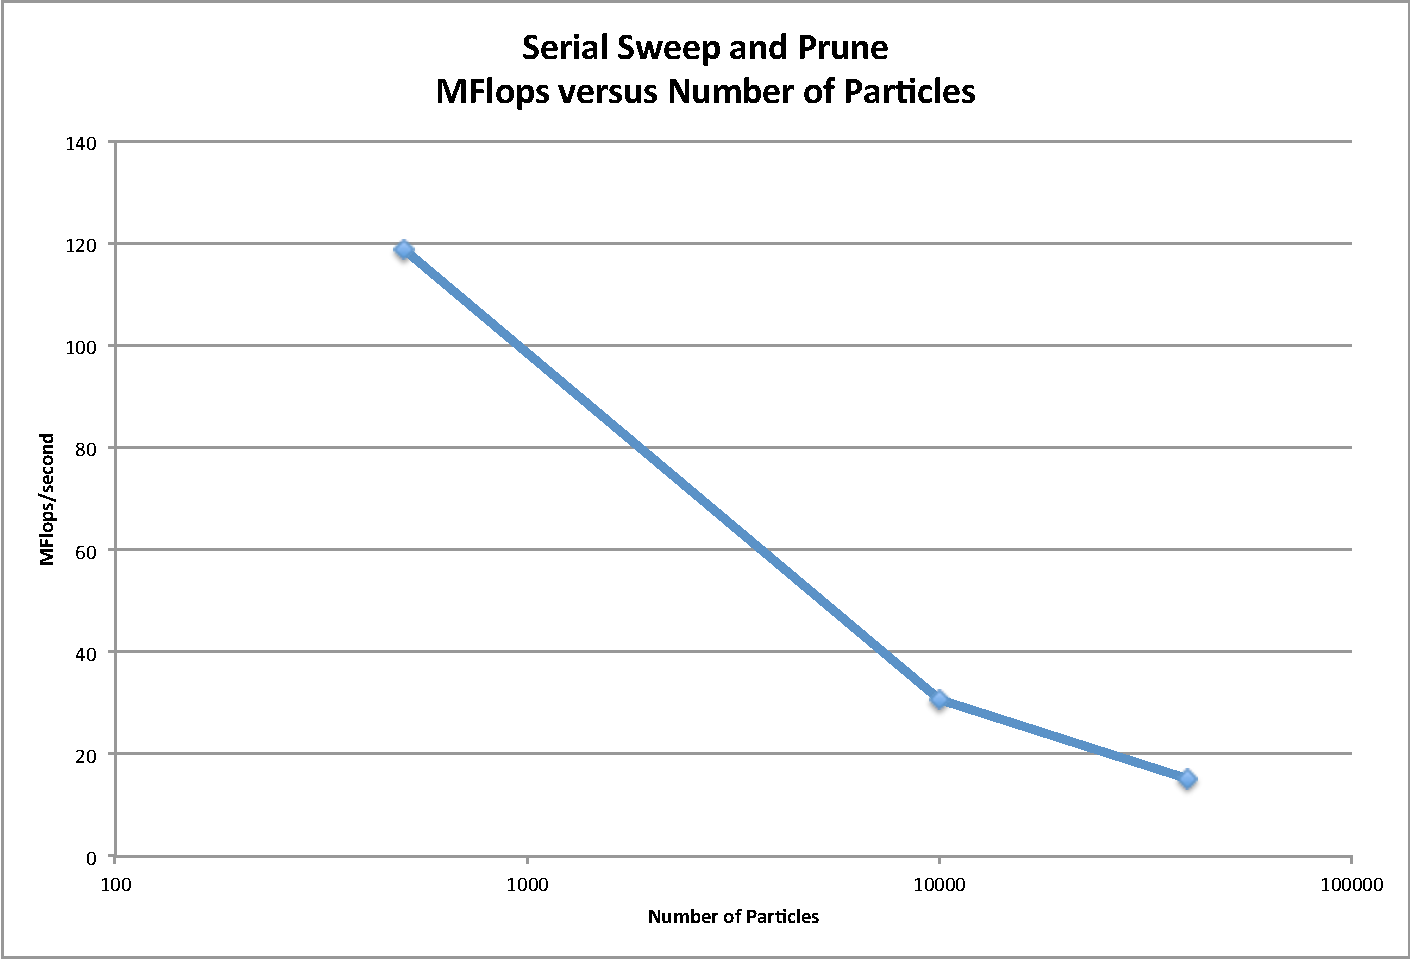
\includegraphics[width=0.5\paperwidth]{figures/serial_flops_v_n}
\par\end{centering}

\caption{Serial Sweep and Prune. MFlops/sec versus Number of Particles.}
\label{plot:serial_flops_v_n}
\end{figure}


\subsection{MPI using Micro-blocks}

Figure~\ref{mpi_mb_n} shows the MPI microblocks implementation follows O(n) for various p. Similar to OpenMP, the same phenomena for higher n with low p and lower n with high p manifest for the same reasons (although here amplified in magnitude due to the larger problem space explored). Figure~\ref{mpi_mb_p} demonstrates the MPI microblocks implementation scales by O(n/p) as desired. The scaling for one million particles versus p most visibly demonstrates the power of the MPI implementation to exploit parallelism in this problem. In fact, since the MPI implementation strictly partitions the memory (compared to OpenMP), superscaling better than 1/p is exhibited as increasing p reduces the impact of memory issues. Even so, overhead costs from communication and synchronization limit the number of cores usable for sub-million particle problems to 48.

\begin{figure}[!h]
\centering
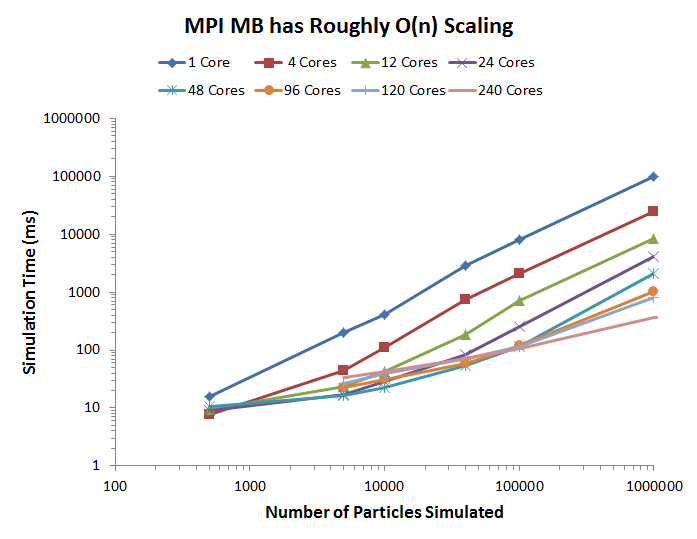
\includegraphics[width=0.7\textwidth]{figures/mpi_mb_n.png}
\caption{}
\label{mpi_mb_n}
\end{figure}

\begin{figure}[!h]
\centering
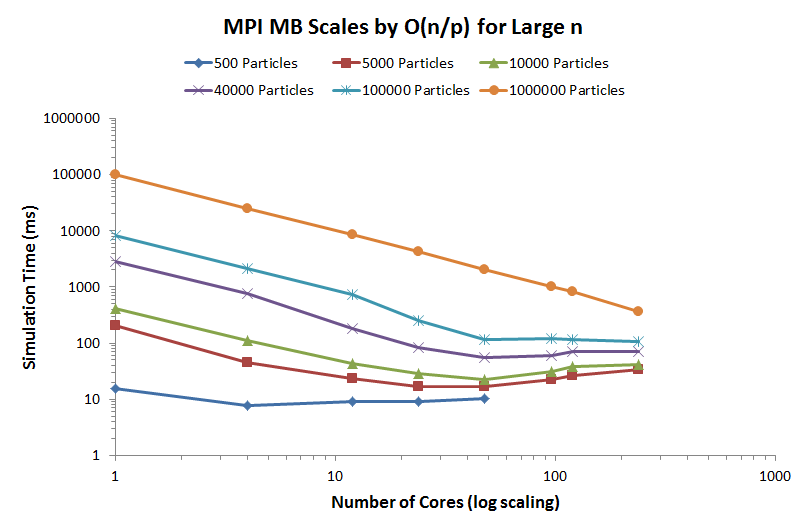
\includegraphics[width=0.7\textwidth]{figures/mpi_mb_p.png}
\caption{}
\label{mpi_mb_p}
\end{figure}

Figure~\ref{mpi_mb_flops} explores how computational intensity (measured using IPM) changes as a function of the n and p. For very small n, the overhead in MPI communication causes lower p to be favored. However, for a million particles, the overhead is effectively hidden by the computation size thus allowing for good performance scaling with p. For `medium' n, 24-48 cores form a sweet spot balancing increasing MPI overhead with decreasing memory footprint and thus deliver the best performance. Figure~\ref{mpi_mb_rtime}, which graph the relative time spent synchronizing, computing, and communication, sheds some light on these results. The optimal performance is gained when slightly more than half the time is spent computing. In general, the time spent synchronizing tracks the time spent communication (likely since synchronization waits are only incurred immediately following communication steps to ensure buffers are not overwritten).

\begin{figure}[!h]
\centering
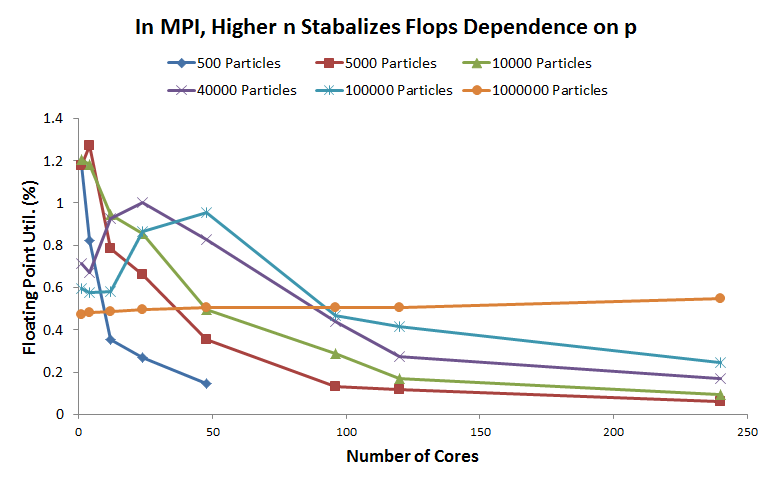
\includegraphics[width=0.8\textwidth]{figures/mpi_mb_flops.png}
\caption{}
\label{mpi_mb_flops}
\end{figure}

\begin{figure}[!h]
\centering
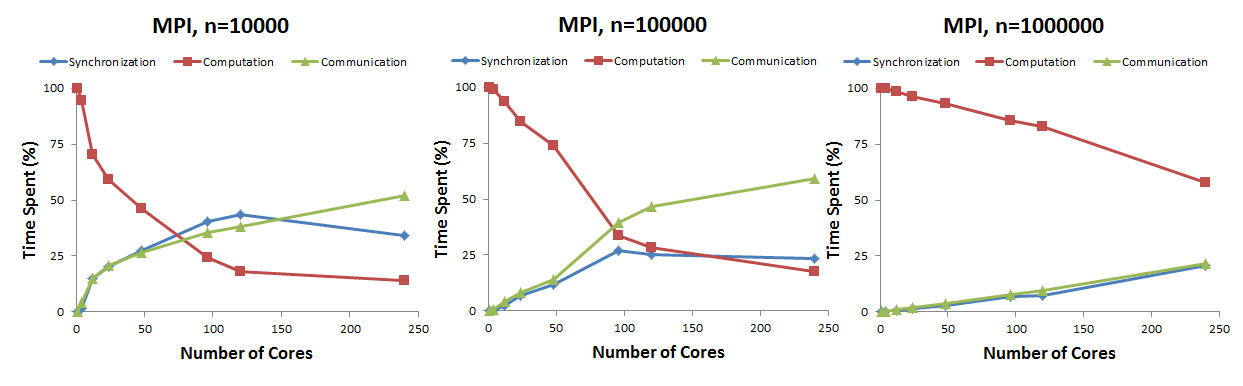
\includegraphics[width=1\textwidth]{figures/mpi_mb_rtime.png}
\caption{}
\label{mpi_mb_rtime}
\end{figure}

\subsection{MPI using Sweep and Prune}

Figure \ref{mpips_time_vs_n} shows the time taken to execute 100 cycles of the simulation, with different numbers of particles (n). Log-log plots for 4, 8, 16, 24 and 48 processors are given. Since each of Hopper's nodes have 24 processors, only the 48-processor plot spans two physical machines; the other experiments were all run on a single machine.

If the MPI Sweep and Prune algorithm ran in purely O(n) time, one would expect the log-log curves in Figure~\ref{mpips_time_vs_n} to be linear with a slope of 1. However, if one attempts to fit a polynomial curve to these plots, one finds that the degree of linearity depends on the number of processors. With 4 processors, the time versus n curve is best approximated by an O(n$^{1.7}$) curve, while at 24 processors, the curve is best approximated by a straight line, i.e. O(n). Therefore, the algorithm runs in O(n) time, as long as 16 or more processors are used in parallel. The O(n$^{1.7}$) run-time with few processors is due to the O(n$^{2}$) sort that must be performed whenever a ghost particle or immigrant particle is inserted into a local processor's particle list. With 16 or more processors, the number of immigrants and ghosts per processor decreases sufficiently that this sorting cost becomes negligable.

\begin{figure}[!h]
\centering
\includegraphics*[width=0.7\textwidth, viewport= 70 70 730 550]{figures/mpips_time_vs_n}
\caption{}
\label{mpips_time_vs_n}
\end{figure}

Figure \ref{mpips_speedup_vs_p} is a log-linear plot showing the percentage of peak machine FLOPS/s acheived as the number of processors is increased. For all values of {\em n} and {\em p}, the parallel algorithm does not acheive more than 1\% of total machine peak (i.e. combined performance of all processors). This clearly indicates that the software is spending a large amount of time waiting for MPI network responses or cache misses. Furthermore, the percentage of machine peaks seems to decreases slightly as P increases, indicating that the algorithm spends more time communicating and less time computing, as the number of processors is increased. This is verified by Figure~\ref{mpips_timealloc_vs_p}.

Other than these facts, not much else can be drawn from this plot, due to the unreliable FLOPS/s reported by Craypat. Craypat introduces a large overhead when profiling the code (as large as 99\%), which must be factored out in the FLOPS/s calculation. However, the exact overhead is only an estimate, and varies drastically from run to run. As a result, the curves in Figure \ref{mpips_speedup_vs_p} are rather noisy. This could be improved by profiling the code multiple times, and averaging the results.

\begin{figure}[!h]
\centering
\includegraphics*[width=0.7\textwidth, viewport= 70 70 730 550]{figures/mpips_flops_vs_p}
\caption{}
\label{mpips_flops_vs_p}
\end{figure}

Figure \ref{mpips_speedup_vs_p} shows the speedup achieved by adding more processors. Note that this is relative to the purely serial sweep-and-prune code, which does not do any communication. For 500 particles, no speedup is achieved by adding more processors, as the processors spend all their time communicating and virtually no time actually computing collisions. However, for 10 000 particles, the speedup curve is perfectly linear with a slope of 1. If the number of processors is doubled, the program runs in half the time. However, the speedup is not {\em p-times}, but rather {\em (p/k)-times}, where {\em k} is the fixed cost of communication. At a count of 40 000 processors, the speedup is actually greater than linear, as the number of ghost and immigrant particles per processor decreases as {\em p} is increased. Since the cost of sorting the ghost and immigrant particles into the local particle list is costly, increasing the number of processors has a big effect on reducing this cost.

\begin{figure}[!h]
\centering
\includegraphics*[width=0.7\textwidth, viewport= 70 70 730 550]{figures/mpips_speedup_vs_p}
\caption{}
\label{mpips_speedup_vs_p}
\end{figure}

Figure~\ref{mpips_timealloc_vs_p} shows how execution time is allocated for simulating 10 000 particles on different numbers of processors. As the number of processors is increased, each processor does less computation per cycle. However, the number of MPI messages sent by each processor is constant. Therefore, as {\em p} increases, a smaller portion of the time is spent computing, and a greater portion is spent communicating. The synchronization curve indicates the time spent in the MPI {\em Waitall} operation. This is always almost 0\%, as the actual synchronization is performed by the blocking MPI receive calls.

\begin{figure}[!h]
\centering
\includegraphics*[width=0.7\textwidth, viewport= 70 70 730 550]{figures/mpips_timealloc_vs_p}
\caption{}
\label{mpips_timealloc_vs_p}
\end{figure}

\subsection{Pthreads using Sweep and Prune}
Figure \ref{plot:thread_t_v_n} shows how the execution time scales
with the number of particles for varying numbers of processors, $p=4,8,16,\text{ and }24$.
Results are shown on a log-log plot. The plot clearly captures the
amount of overhead involved with parallelization and the intersections
of the lines show the cross-over point for the number of particles
at which it is beneficial to increase to the next level of parallelism. 

\begin{figure}
\begin{centering}
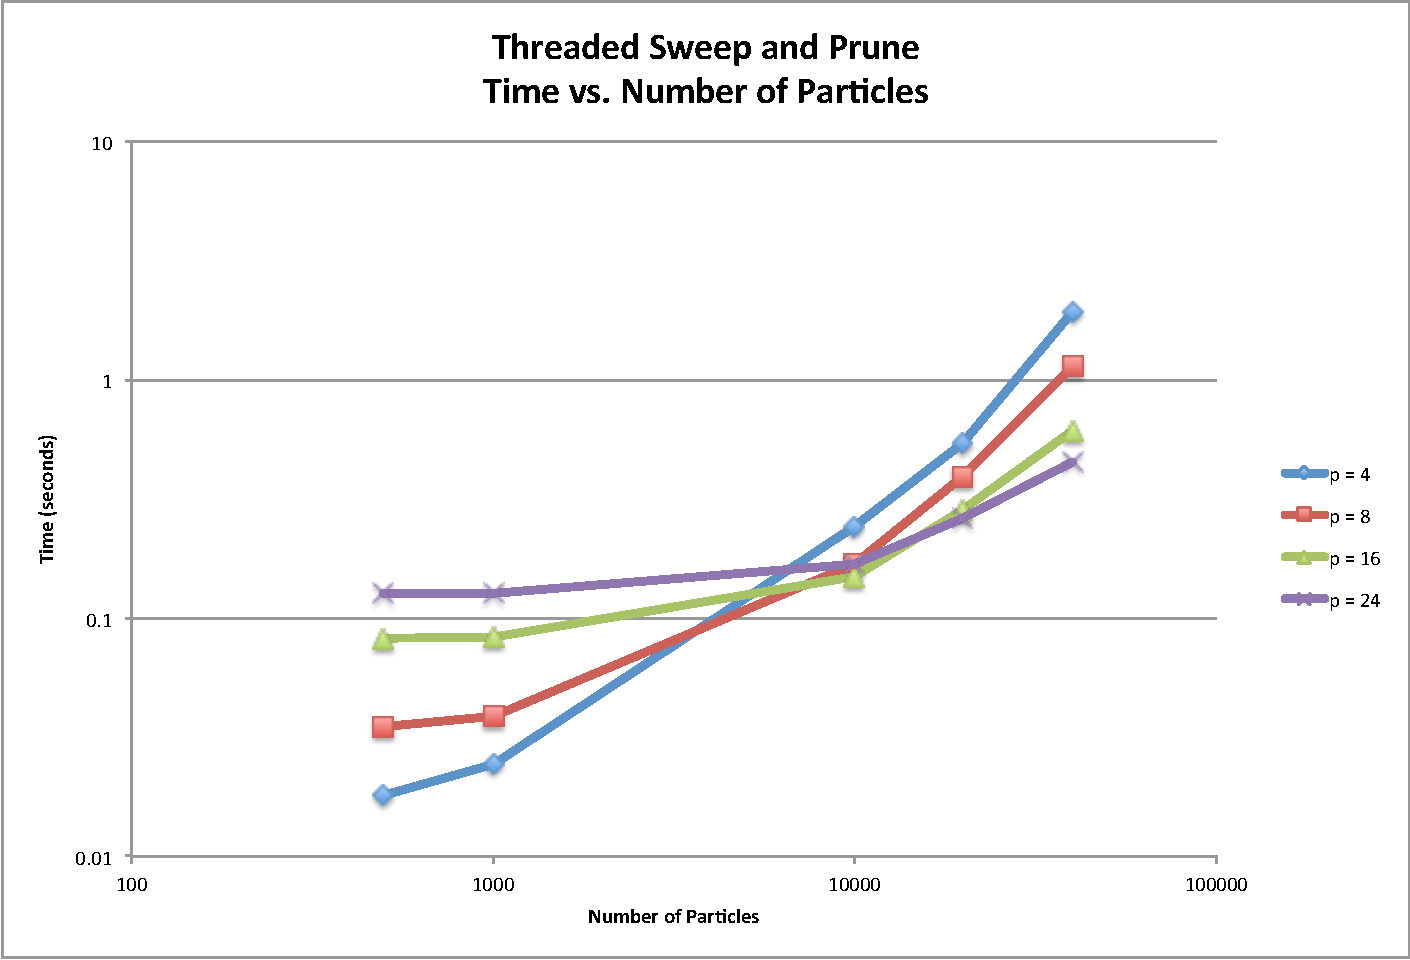
\includegraphics[width=0.5\paperwidth]{figures/thread_t_v_n}
\par\end{centering}

\caption{Threaded Sweep and Prune. Time versus Number of Particles.}
\label{plot:thread_t_v_n}
\end{figure}


Figure \ref{plot:thread_speedup_v_p} shows the speed up in terms
of execution time of the threaded prune and sweep code over the serial
code. Because of the overhead involved in keeping track of particle
regions and ghost particles, the threaded version starts off slower
than the serial version for small numbers of particles. However for
large numbers of particles, $n=40000$, we see a consistent linear
speedup as we increase the number of processors. For a medium number
of particles, $n=10000$, we see a speed up until $p=16$ at which
point the communication costs dominate. 

\begin{figure}
\begin{centering}
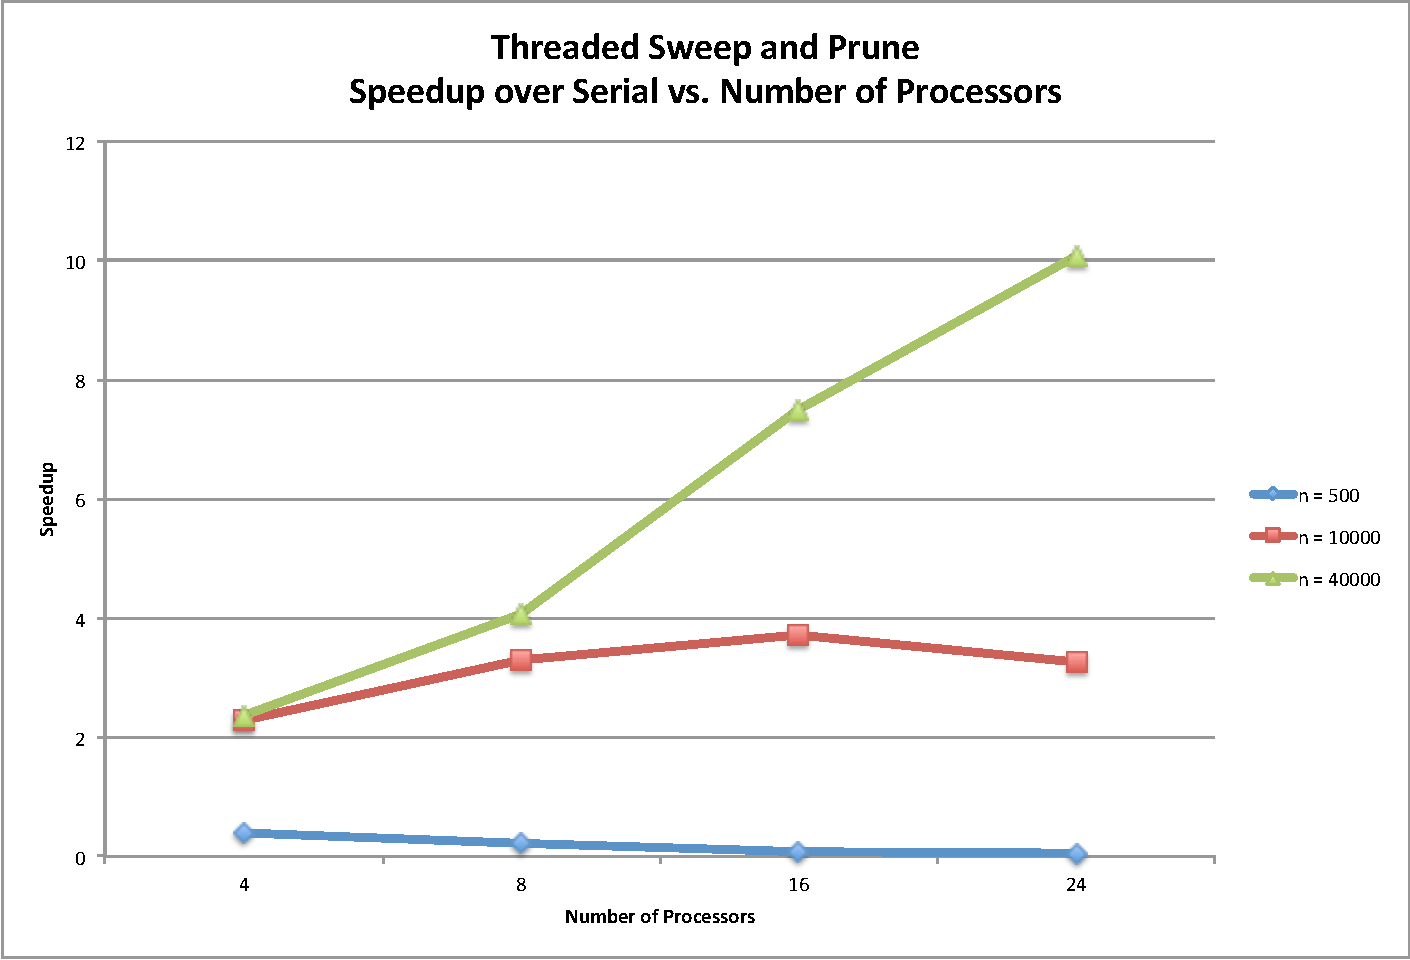
\includegraphics[width=0.5\paperwidth]{figures/thread_speedup_v_p}
\par\end{centering}

\caption{Threaded Sweep and Prune. Speed up over serial versus Number of Processors.}
\label{plot:thread_speedup_v_p}
\end{figure}


Figure \ref{plot:thread_flops_v_p} shows how the number of floating
point operations scales with the number of processors. As the number
of processors increase the arithmetic intensity decreases indicating
that the communication and synchronization costs are dominating the
computation. We note that the arithmetic intensity for a small number
of processors for $n=10000$ particles starts out higher than for
$n=40000$ particles. This is due to the amount of time spent performing
collision detection versus performing force and position updates. 

\begin{figure}
\begin{centering}
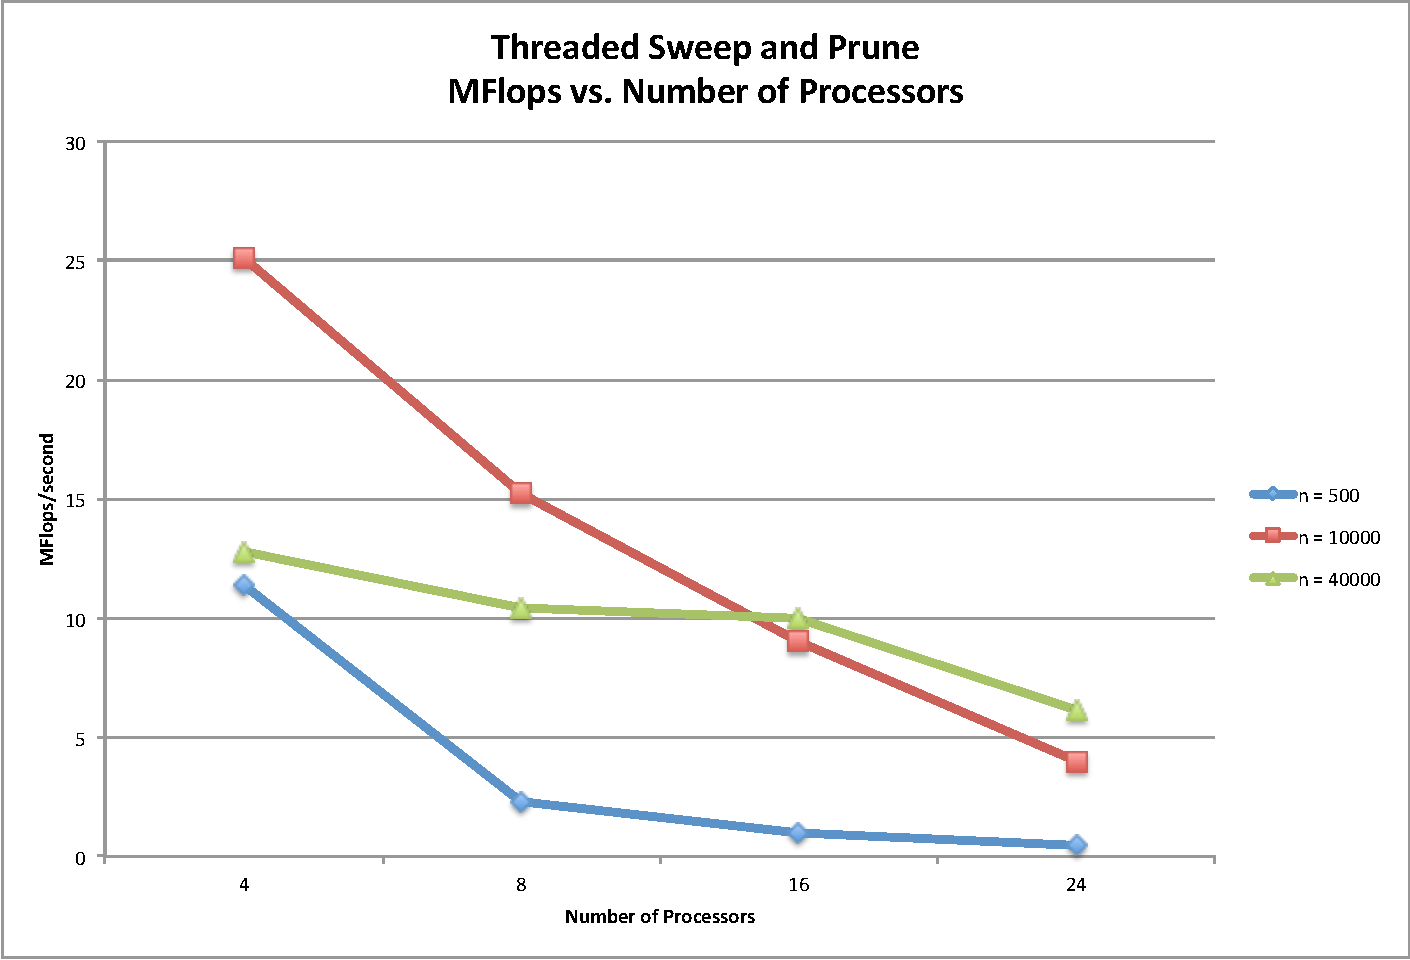
\includegraphics[width=0.5\paperwidth]{figures/thread_flops_v_p}
\par\end{centering}

\caption{Threaded Sweep and Prune. MFlops/second versus Number of Processors.}
\label{plot:thread_flops_v_p}
\end{figure}


Figure \ref{plot:thread_breakdown_10000} shows a breakdown of the
execution time in terms of time spent doing computation, communication,
and synchronization. For the threaded implementation, communication
is defined as the time spent copying particle data from one region
to another. Synchronization is defined as the amount of time spent
waiting for threads to arrive at the same barrier. Computation is
defined as the rest of the execution time that is not communication
nor synchronization. We see that actual communication costs are negligible
compared to synchronization costs. This may be due to our implementation
choice of allowing regions to accept particles from only one thread
at a time. This scheme requires 8 barriers to transmit ghost particles
to neighbouring regions, as one barrier is needed after each send
to the N, NE, E, SE, S, SW, W, and NW neighbours. 

\begin{figure}
\begin{centering}
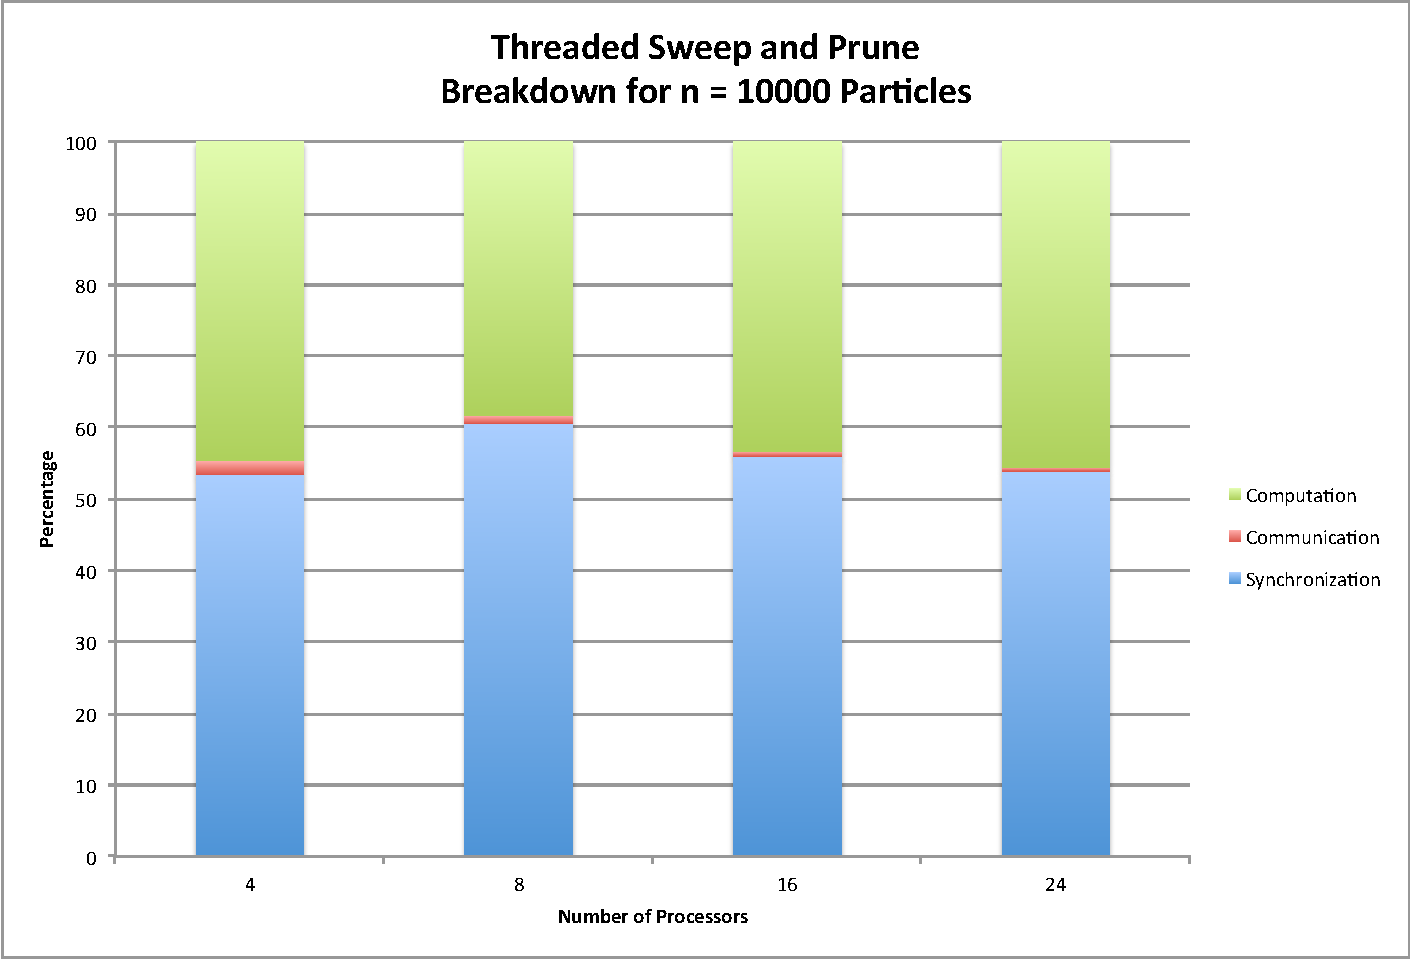
\includegraphics[width=0.5\paperwidth]{figures/thread_breakdown_10000}
\par\end{centering}

\caption{Threaded Sweep and Prune. Breakdown of Execution Time versus Number
of Processors.}
\label{plot:thread_breakdown_10000}
\end{figure}

\subsection{OpenMP using Micro-blocks}

Figure~\ref{openmp_mb_n}  demonstrates the OpenMP microblocks implementation also scales roughly with O(n). When p is low, performance scales very precisely as O(n) for low n whereas for higher p, performance scales with O(n) for higher n. The former phenomenon is explained by overhead and synchronization needed by OpenMP using many threads that is exposed at low n. The latter phenomenon can again be explained by memory effects: when p is higher, more memory caches are available thus allowing the handling of higher n. Figure~\ref{openmp_mb_p} demonstrates that the OpenMP implementation scales by O(n/p) when n$\geq$10000 and p$\leq$12. The boundary at 12 corresponds with known features of the Hopper architecture: the system is composed of 12-core processors. When the number of cores used increases above 12, requests must now be serviced on a larger interconnect network, incurring higher overhead. Due to the leveling off with p in this figure, OpenMP was not even attempted for p$>$24.

\begin{figure}[!h]
\centering
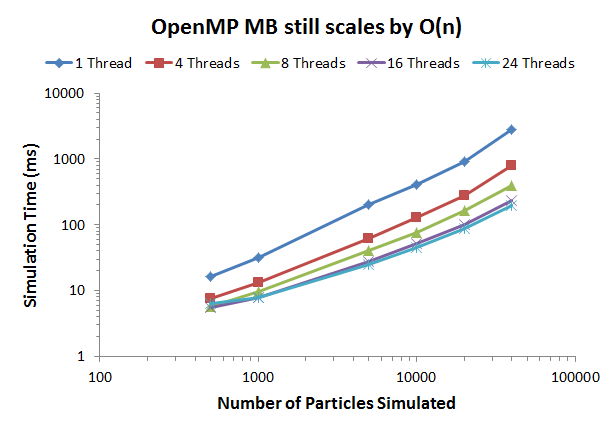
\includegraphics[width=0.7\textwidth]{figures/openmp_mb_n.png}
\caption{}
\label{openmp_mb_n}
\end{figure}

\begin{figure}[!h]
\centering
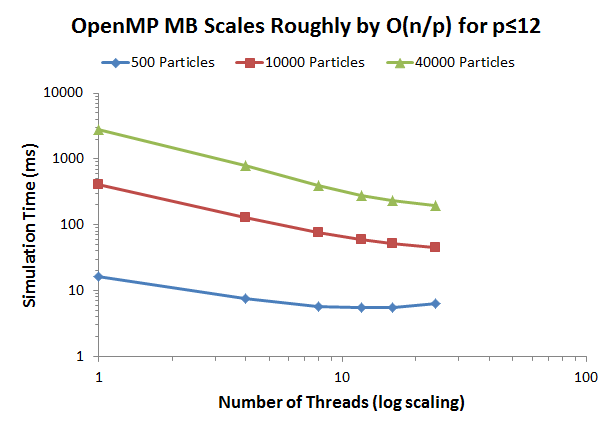
\includegraphics[width=0.7\textwidth]{figures/openmp_mb_p.png}
\caption{}
\label{openmp_mb_p}
\end{figure}

Figure~\ref{openmp_mb_flops} shows that the floating point utilization (measured using CrayPAT) drops as the number of threads increases. Again, this is likely due to memory effects. However, in contrast to the serial implementation where memory issues generally equated to cache misses, here the slowdown from memory operations is attributable to cache coherence overhead amongst the system cores. Figure~\ref{openmp_mb_rtime} tracks the time spent in portions of particle simulation (for select n) versus p. Somewhat surprisingly, the portion of time spent handling particle migrations is constant across both problem size and number of threads used (even though this is the only portion of code using locks). The rise in relative time spent handling movements is most likely a symptom of memory overhead since the actual computation is very simple thus most time is spent dealing with memory. Also, the OpenMP worker threads are redistributed within each compute portion (to help maintain a fair workload as particles move around), thus taxing the cache coherence system.

\begin{figure}[!h]
\centering
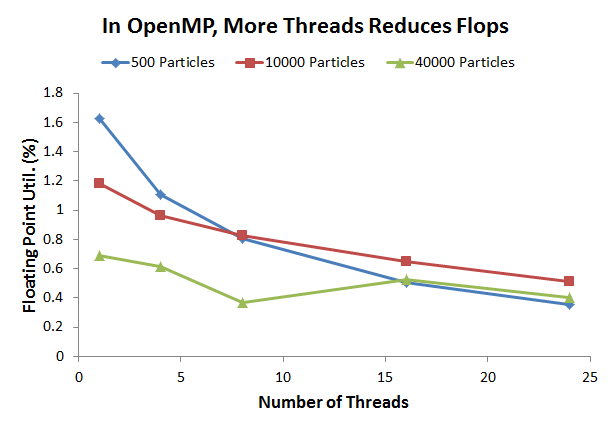
\includegraphics[width=0.7\textwidth]{figures/openmp_mb_flops.png}
\caption{}
\label{openmp_mb_flops}
\end{figure}

\begin{figure}[!h]
\centering
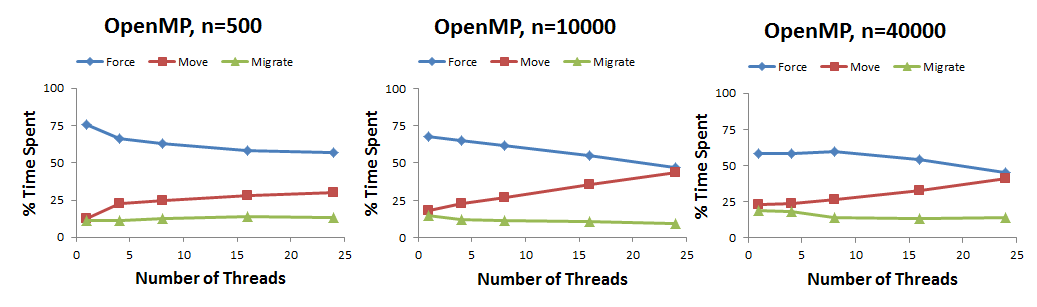
\includegraphics[width=1\textwidth]{figures/openmp_mb_rtime.png}
\caption{}
\label{openmp_mb_rtime}
\end{figure}

\subsection{CUDA using Micro-blocks}

Figure~\ref{gpu_time_vs_n} shows the execution time of the particle simulation algorithm, running on a GPU, for different numbers of particles. The optimized algorithm is asymptotically faster than the naive O(n$^2$) algorithm. At 1000 particles, it is 30 times faster, while at 10 000 particles, it is 330 times faster. On a linear-linear plot, the execution time curve of the optimized algorithm is seen to be linear, with a gradient of 8$\mu$s/particle.

\begin{figure}[!h]
\centering
\includegraphics*[width=0.65\textwidth, viewport= 70 70 730 550]{figures/gpu_time_vs_n}
\caption{}
\label{gpu_time_vs_n}
\end{figure}

The plot in Figure~\ref{gpu_time_vs_n} includes all of the positive-effect optimizations described in Section~\ref{gpu-optimization-section}. The individual effect of each of the optimizations is described below:

\begin{itemize}
\item {\em Particle migration: } speedup of 4 times.
\item {\em Single kernel: } a speedup of only 1\%. Since this optimization reduced code readability, it was not used.
\item {\em Vector datatypes and local particle copies: } Speedup of 1.5 times.
\item {\em Per-particle threads for calculating forces: } speedup of 2 times.

\end{itemize}

\subsection{Performance Comparison of all Algorithms}

Serial sweep and prune is faster than serial micro-blocks for n$<$10 000. When n$\geq$10 000, the serial micro-blocks code is faster. This is because the sweep and prune algorithm is extremely efficient at detecting collisions when n is small, but when n is large, the O(n$^2$) sort balloons.

The two MPI variants (prune and sweep, and microblocks) have similar performance for 500 and 1000 particles at all values of n. For more than 1000 particles, the micro-blocks variant is generally faster. The exception is when the number of processors is large, and hence number of particles per processor is small, as this reduces the amount of sorting that needs to be done on each processor. Both MPI variants are faster than the serial versions, as long as the total number of particles is greater than 500. If there are 500 particles or less, the serial code is faster, as there is insufficient computation to compensate for the MPI communication overhead.

The OpenMP implementation, using microblocks, is faster than the Pthreads implementation, which uses prune and sweep, for all particle and processor counts. However, the MPI microblocks implementation still outperforms the OpenMP implementation. This is due to three reasons:
\begin{enumerate}
\item The MPI libraries for Hopper are able to handle intra-node messages fairly efficiently
\item The MPI programming model also strict memory partitioning between nodes
\item The OpenMP model relies on coherence protocols to move microblock and particle data between cores for processing as necessary. 
\end{enumerate}
Thus, compared to MPI, OpenMP must transmit far more data between cores for the same n and p$>$1.

The OpenMP implementation required only 20 additional lines of code to the serial microblocks program, while the MPI microblocks implementation required significant amounts of design, programming, and debugging time. Thus the OpenMP implementation is still competitive, as it allows significant speedups with minimal coding effort, as long as p is small. Considered together, the MPI and OpenMP results motivate a future solution where MPI is used for major region blocking and OpenMP is used for microblocks on a single node.

\section{Discussion and Conclusion}
\label{conclusion-section}

\subsection{The Strengths and Weaknesses of the GPU Architecture}
Optimization of our GPU implementation was significantly more difficult
than our CPU implementations. This is due, in part, to the requirement
for more explicit handling of both memory and execution. For example,
\begin{itemize}
\item The need to manually manage threads and thread blocks and understand
how they map to underlying warps. For this reason, uses of loops and
branches come with a considerable penalty and need to be carefully
managed.
\item The need to manually synchronize and transfer data with the CPU.
\item The need to manually manage the memory hierarchy. The CPU's automatically
managed cache was convenient for obtaining good performance with a
small amount of work. In contrast, the GPU needs to be explicitly
told to store data in fast memory, and transferring data between slow
and fast memory must also be managed manually. We appreciated the
control this allows us over data placement, but at the same time,
missed the convenience of having an automatically handled cache.\end{itemize}

\subsection{Final Conclusions}

\end{document}
